\documentclass{article}

\usepackage{graphicx}
\usepackage{amsmath}

\usepackage[parfill]{parskip}

\title{$k$-d tree}
\author{Gerard Martin Teixidor}

\begin{document}
\maketitle

\section*{Description}
A $k$-d tree~\cite{kd-tree} is a data structure used to store points in a k-dimensional space. Its implementation relies on a binary tree in which every non-leaf node represents a space partition. Each level of the tree is associated with one of the $k$ dimensions which, at each node, splits the space into two subspaces. These two subspaces are represented by the left and right subtrees.

\section*{Implementation}
This $k$-d tree has been implemented using generics. This allows a user defined type to represent the elements (points) which are going to be stored.

It is important to note that this implementation of a $k$-d tree does not grantee that the tree is always balanced. A balancing algorithm could be implemented with a $O(kn~log~n)$ time complexity by using the median~\cite{balanced}.

The data structure code has been programed using the \textit{C++17} and the \textit{GNU Compiler Collection}.

\subsection*{Operations}
List of the allowed operations with a brief description and their time complexity:

\paragraph*{\textit{empty}} Test whether the collection is empty.
\begin{description}
\item[] Time complexity: $O(1)$
\end{description}

\paragraph*{\textit{size}} Return the collection size.
\begin{description}
\item[] Time complexity: $O(1)$
\end{description}

\paragraph*{\textit{insert}} Insert an element.
\begin{description}
\item[] Time complexity: $O(log~n)$ 
\end{description}

\paragraph*{\textit{erase}} Erase an element.
\begin{description}
\item[] Time complexity: $O(log~n)$ 
\end{description}

\paragraph*{\textit{clear}} Erase all elements.
\begin{description}
\item[] Time complexity: $O(1)$
\end{description}

\paragraph*{\textit{contains}} Test whether the collection contains an element.
\begin{description}
\item[] Time complexity: $O(log~n)$ 
\end{description}

\paragraph*{\textit{min}} Return the element with the minimum dimension.
\begin{description}
\item[] Time complexity: $O(n)$ 
\end{description}

\paragraph*{\textit{range}} Return the elements that are inside a given range.
\begin{description}
\item[] Time complexity: $O(log~n + m)$ where $m$ is the number of reported points.
\end{description}

\paragraph*{\textit{nearest\_neighbor}} Return the nearest neighbor element of a given element.
\begin{description}
\item[] Time complexity: $O(log~n)$ 
\end{description}

\paragraph*{\textit{operator\textless\textless}} Inserts the tree string representation into an output stream.

\section*{Experiments}
To test the time complexity of the data structure two experiments have been performed. Note that, in both tests, the results have variability. This is due unbalanced nature of the data structure. Another explanation is the memory management by the operative system since this implementation does not preallocate memory when the collection is created. In both experiments the outliers have been removed by using a handpicked quartile.

The fist experiment (Figure:~\ref{fig:insert}) shows that, in effect, the time complexity of the \textit{insertion} operation is $O(log~n)$. As in the previous experiment, this second experiment (Figure:~\ref{fig:contains}) shows that the  \textit{contains} (search) operation also follows a logarithmic order.

\begin{figure}
\centering
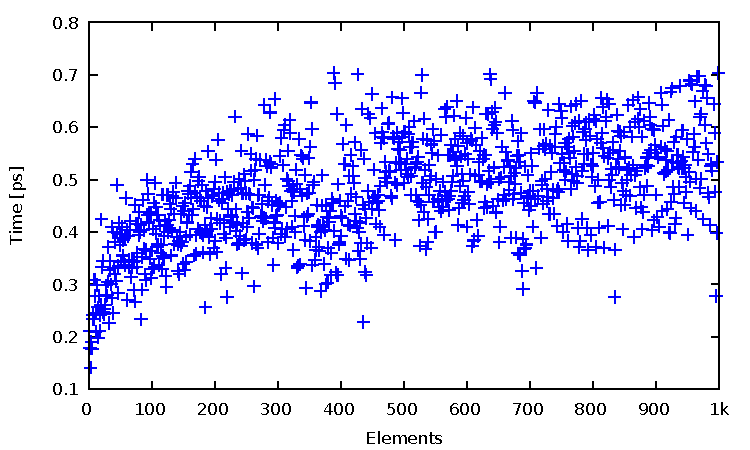
\includegraphics[width=\linewidth]{insert_outlayers.pdf}
\caption{Plot showing the \textit{insert} operation $O(log~n)$ time complexity.}
\label{fig:insert}
\end{figure}

\begin{figure}
\centering
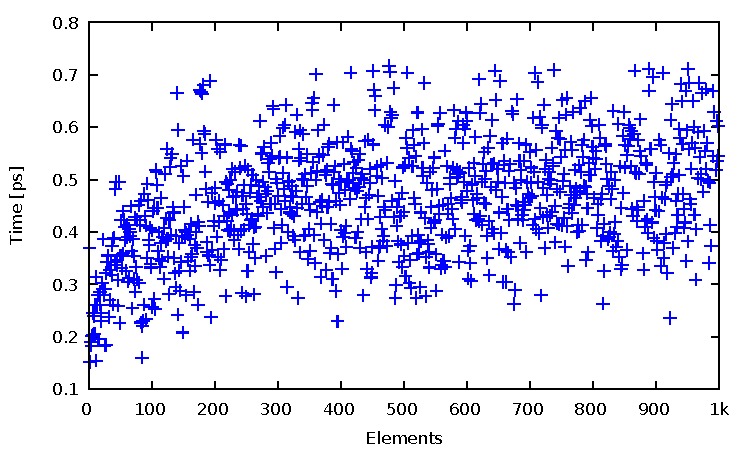
\includegraphics[width=\linewidth]{contains_outlayers.pdf}
\caption{Plot showing the \textit{contains} operation $O(log~n)$ time complexity.}
\label{fig:contains}
\end{figure}

\bibliographystyle{unsrt}
\bibliography{report.bib}


\end{document}